% Osdag Design and Detailing Check List (DDCL)
% Beam to Column End Plate Moment Connection 
% Author: Ajmal Babu M S
\documentclass[11.5pt,a4paper,oneside]{report}
\usepackage{graphicx}
\usepackage{url}
\usepackage{palatino}
\usepackage{tabularx}
\fontfamily{SansSerif}
\usepackage[T1]{fontenc}
%\usepackage[T1]{fontenc}
%\usepackage[latin1]{inputenc}
\usepackage{amsmath}
\usepackage{amsfonts}
\usepackage{amssymb}
%\usepackage{graphicx}
\usepackage{siunitx}
%\usepackage{tabularx}
\usepackage{algorithm2e}
\usepackage[top=1in, bottom=1in, left=0.8in, right=0.6in]{geometry}
\usepackage{fancyhdr}
%\usepackage{fancyheadings}
\usepackage{multirow}
\usepackage[bookmarks=false]{hyperref}   % For creating hyperlinks

\makeatletter
\makeatother
\hypersetup{
    colorlinks=true,
    linkcolor=blue,
    filecolor=magenta,      
    urlcolor=blue,
}
%======================================================
%					New Commands
%++++++++++++++++++++++++++++++++++++++++++++++++++++++
% To make the manual calculaion document, comment out following section
% and uncomment next section.
%------------------------------------------------------
%\newcommand{\okornot} { 
%	\vspace{15mm} \hrule \vspace{5mm}
%	\underline{Calculations} \\ \\ \noindent 
%	\TextField[name=multilinetextbox, multiline=true, width=1.0\linewidth,height=4in]{}} 
%------------------------------------------------------
\newcommand{\okornot}{ \vspace{15mm} \hrule
	\noindent \\ \\
	Is this check \qquad
	\CheckBox[checked=False, name= ok]{\textbf{Ok}} \qquad / 
	\CheckBox[checked=False, name= notok]{\textbf{Not Ok}}\\ \\
	Comments \\ \\
	\noindent
	\TextField[name=multilinetextbox, multiline=true, width=1.0\linewidth,height=2in]{}}
%++++++++++++++++++++++++++++++++++++++++++++++++++++++
% References for the check
\newcommand{\checkrefernces} {
	\vspace{15mm} \hrule \vspace{2mm}
	\textit{References:}}
%++++++++++++++++++++++++++++++++++++++++++++++++++++++
% Change 'Chapter' to 'Check'
\renewcommand{\chaptername}{Check}
%======================================================
%------------------------------------------------------
\begin{document}
	\title{Osdag\\ Open steel design and graphics}
	\author{Ajmal Babu M S}
	\date{07 August 2018}
\pagestyle{fancy}
\lhead{}
\chead{}
\rhead{\bfseries Moment Connection Module}
\lfoot{Osdag - Open steel design and graphics}
\cfoot{}
\rfoot{\thepage}
\renewcommand{\headrulewidth}{2pt}
\renewcommand{\footrulewidth}{1pt}
\newcommand{\univ}{Indian Institute of Technology, Bombay}
%------------------------------------------------------
\begin{titlepage}
	\begin{center}
		\begin{center}
			
\includegraphics {logoOsdag.png}
		\end{center}
			{\LARGE {Design and detailing checklist (DDCL)}}\\
			\vspace{1cm}
			{\LARGE {Beam to column end plate  moment connections}} \\
			\vspace{1cm}		
			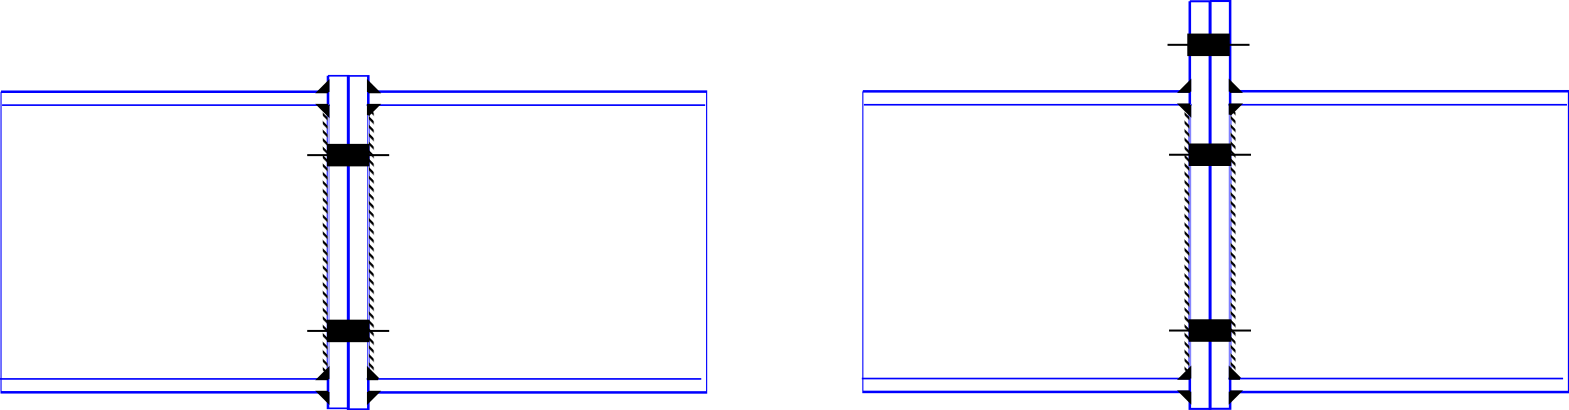
\includegraphics[width=7in]{FP_OWE.png} \\	
			\vspace{3cm}
			 {\small {Prepared by:}} \\
			 {\Large \textbf {Ajmal Babu M S}} \\	
			\vspace{0.5cm}	
			{\small {Under the guidance of} }\\
			{\Large \textbf {Prof. Siddhartha Ghosh}} \\	
			\vspace{1cm}
			\centering
			
\includegraphics[width=1.2in]{logo.png} \\	
 			\vspace{0.5cm}
			{\univ} \\ 
			\vspace{0.15cm}		
			{August 2018}
	\end{center}
\end{titlepage}
%------------------------------------------------------
\tableofcontents
\begin{Form}
%------------------------------------------------------
\pagenumbering{arabic}
\chapter*{Guideline for filling DDCL}
	\begin{itemize}
			\item    Guideline1
			\item    Guideline2
	\end{itemize}
%------------------------------------------------------
\chapter*{Reviewer Details}

%------------------------------------------------------
\chapter*{User Inputs}


\begin{itemize}
	
	\item Connecting members
	\begin{itemize}
		\item Connectivity*
		\item Beam Section*
		\item Column Section*
		\item fu (MPa)* 
		\item fy (MPa)* 
		
	\end{itemize}

	\item Factored loads
		\begin{itemize}
		\item Moment (kNm)*
		\item Vert. Shear (kN)*
		\item Axial Force (kN)
		\end{itemize}
	\item Bolt
		\begin{itemize}
		\item Diameter (mm)*
		\item Type *
		\item Grade *
		\end{itemize}
	\item Plate
		\begin{itemize}
		\item Thickness (mm)*
		\item Height (mm)
		\item Width (mm)
		\end{itemize}
	\item Weld size
		\begin{itemize}
		\item Flange weld (mm)*
		\item Web weld (mm)*
		\end{itemize}
\end{itemize}
%=====================================================
\part*{Design and Detailing Checks}
%------------------------------------------------------
\chapter{Connecting Members}
%
The column and beam are allowed to connect by following connectivites.
\begin{itemize}
	\item Column flange to beam web
	\item Column web to beam web
\end{itemize}
%
The column and beam sections are provided as a dropdown list in Osdag input dock. Tapered sections from IS 808:1989 and parallel flange sections from the upcoming version of IS 808 are included. Old sections are highlighted in red colour in the dropdown with a warning that "user is using an old section which is not available in latest version of IS 808" in the message log.
%\section{Connectivity}
%------------------------------------------------------
%
\section{Column Section}
%
All the columns sections are shown in dropdown.
%------------------------------------------------------
\section{Beam Section}
%
For column flange to beam web connectivity, 
\begin{equation}
	w_{bf} \le w_{cf}
\end{equation}
%
For column web to beam web connectivity,
\begin{equation}
	w_{bf} \le d_c - 2 (t_{cf} + r_{c1} + gap)
\end{equation}
Where, \\
\indent $w_{bf}$ = Width of beam flange \\
\indent $w_{cf}$ =  Width of column flange \\
\indent $d_c$ = Depth of column \\
\indent $t_{cf}$ = Thickness of column flange \\
\indent $r_{c1}$ = Root radius of column \\
\indent $gap$ = Clearance between beam and column flanges, 5mm

\checkrefernces
\begin{enumerate}
	\item IS 808:1989
	\item INSDAG Database for parallel flange sections
\end{enumerate}
\okornot
%------------------------------------------------------
%					Material strength
%------------------------------------------------------
\chapter{Material Strength}
%
The column, beam and end plate are supposed to have the same strengths following the Indian Standards. The grades available in IS 800:2007 and IS 2062:2010 are included with a warning that "user is using a section of grade which is not available in the latest version of IS 2062". The values of material strength will be subjected to the following limits in \textbf{MPa};
	\section{Yield Stress limits}
	\begin{equation}
	250 \leq f_{y} \leq 650
	\end{equation}
	\section{Ultimate Stress limits}
	\begin{equation}
	410 \leq f_{u} \leq 780
	\end{equation}
	
	\checkrefernces
		\begin{enumerate}
			\item Table-1, IS 800 : 2007
			\item Table-2, IS 2062 : 2011
		\end{enumerate}
	\okornot
%------------------------------------------------------
%					Factored Loads
%------------------------------------------------------
\chapter{Factored loads}
%
Factored values of the moment (in kNm) and vertical shear force  (in kN) acting on connection is mandatorily taken from the user. An optional field for axial force (in kN) is also given in the input dock if it is acting.\\
Assuming the beam is laterally supported and factored shear force does not exceed 0.6 times the its design shear strength, 
The minimum moment capacity of connection,
\begin{equation}\label{eq:cl_10.7b, IS 800}
	M_{min} = 0.5 M_d 
\end{equation}
Where, \\
\indent $M_{min}$ = Minimum moment capacity of connection \\
\indent $M_d$ = Design bending strength of beam, given by
\begin{equation} \label{eq:cl_8.2.1.2a, IS 800}
M_d = \beta_b Z_p f_y / \gamma_{m0} \le 1.5 Z_e f_y / \gamma_{m0} 
\end{equation}
Where, \\
\indent $\beta_b$ = 1.0 for plastic and compact sections;\\
\indent $\beta_b$ = $Z_e/Z_p$ for semi-compact sections;\\
\indent $Z_p, Z_e$ = Plastic and elastic section modulii of the cross-section, respectively; \\
\indent $f_y$ = Yield stress of the material; and;\\
\indent $\gamma_{m0}$ = Partial safety factor \\
\indent $M_{min}$ = Minimum moment capacity of connection



\checkrefernces
\begin{enumerate}
	\item cl. 10.7, IS 800:2007 \eqref{eq:cl_10.7b, IS 800} 
	\item cl. 8.2.1.2, IS 800:2007 \eqref{eq:cl_8.2.1.2a, IS 800} 
\end{enumerate}
\okornot
%------------------------------------------------------
%					Bolt
%------------------------------------------------------
\chapter{Bolt}
%
The diameter (in mm), type of bolt action (bearing or friction grip) and grade of bolts are taken from user as inputs.

%------------------------------------------------------
%------------------------------------------------------
%------------------------------------------------------
%					Number of bolts
%------------------------------------------------------

\section{Number of bolts}

\large Number of bolts in the configuration \\
	
	\textbf{Assummption:} \\
	
	The minimum number of bolts required for the flush plate configuration is 4 and that for the extended one way configuration is 6. 
	Also, the flush end plate will be restricted to a maximum 6 number of bolts whereas the extended one way end plate will be restricted to 8 number of bolts.
	
	\vspace{5mm}
					
	Force/tension in the tension flange:
		\begin{equation}
			\boxed{Force = \frac{M}{(D - t_{f})}}
		\end{equation}
		
			where, \\
			$M$ = external factored moment + moment due to axial force \\
			$D$ = depth of beam \\
			$t_{f}$ = thickness of beam flange \\
			
			Number of bolts required at the tension flange
			\begin{equation}
				\boxed{= \frac{Force}{Tension \, capacity\, of\, single\, bolt}} 
			\end{equation}
			Number of bolts (provided) at the compression flange = 2
			
		\checkrefernces
			\begin{enumerate}
				\item Table-1, IS 800 : 2007
				\item Table-2, IS 2062 : 2011
			\end{enumerate}
		\okornot
		

%------------------------------------------------------
%					Detailing
%------------------------------------------------------		
\chapter{Detailing}
		
		{\centering
		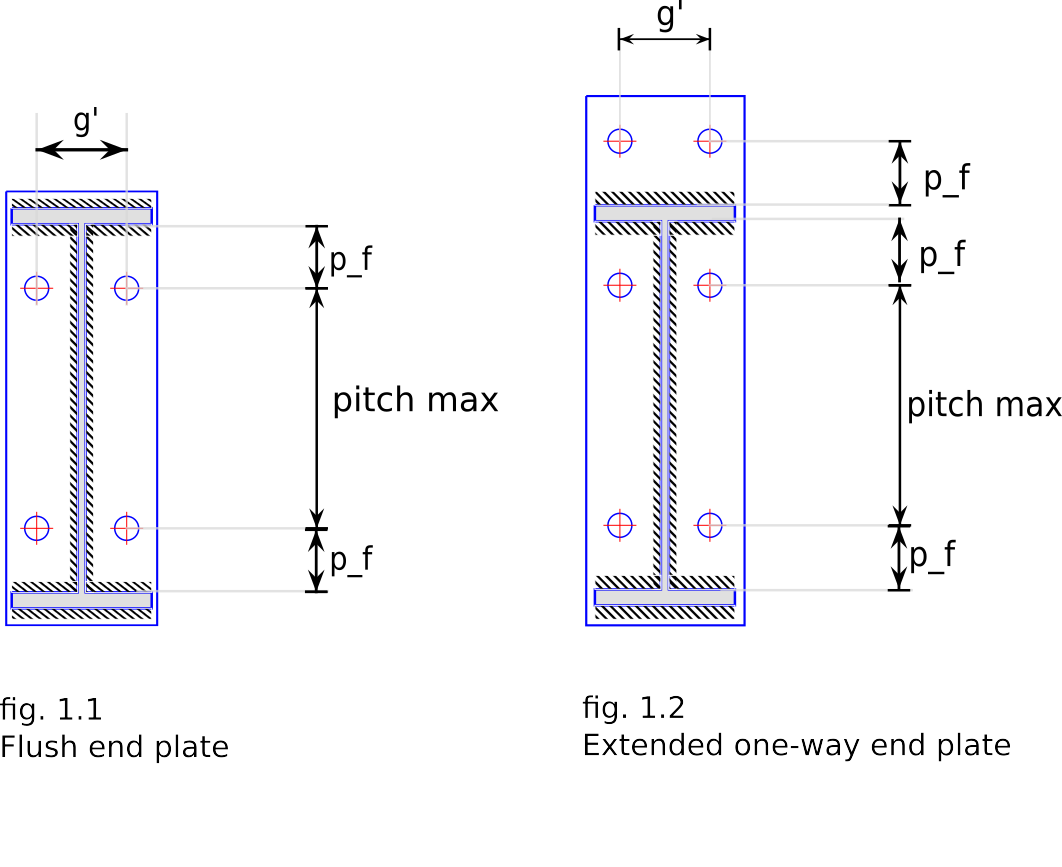
\includegraphics[width=5in]{svg_drawingFPEOW.png} \\}
		
			\begin{enumerate}
				
				\item \large  {Pitch (p)/ Gauge (g) distance (\textbf{already reviewed}) [Reference: Clause 10.2.2 and 10.2.3, IS 800 : 2007]} \\
				%\vspace{5mm}
				\begin{equation}
				\boxed{ 2.5 * bolt\, diameter\, \leq \textbf{\,pitch/gauge \,} \leq min(32 * t,\, 300\, mm) }
				\end{equation}
				
				\hspace{10mm}
				where,
				
				\hspace{30mm}
				t = thickness of thicker plate being connected 
				
			\vspace{2mm}
				
				\item \large {End (e)/ Edge (e') distance (\textbf{already reviewed}) [Reference: Clause 10.2.4, IS 800 : 2007]} \\
				%\vspace{5mm}
				\begin{equation}
				\boxed{ 1.7 * bolt\,hole\, diameter\, \leq \textbf{\,end/edge \,} \leq 12*t*\varepsilon }
				\end{equation}
				
				\hspace{10mm}
				where,
				
				\hspace{30mm}
				t = thickness of thicker plate being connected
				
				\hspace{30mm}
				$\varepsilon = (250 / f_{y}) ^ {(1/2)}$ 
				
				\hspace{30mm}
				$f_{y}$ = yield strength of beam/plate material 				 
			
			\vspace{2mm}
				
				\item \large {Cross-centre gauge distance (g')} (\textbf{refer fig. 1.1 and 1.2}) \\
					\begin{enumerate}
						\item Flush end plate. [Reference: AISC Design Guide - 16, table 3-6, page 22]
						\begin{equation}
						\boxed{ 57 mm \leq \textbf{g'} \leq 95 mm }
						\end{equation}
						
						\item Extended one way. [Reference: AISC Design Guide - 16, table 4-7, page 39]
						\begin{equation}
						\boxed{ 69 mm \leq \textbf{g'} \leq 177 mm }
						\end{equation}
					\end{enumerate}
					
				
			\vspace{5mm}
\okornot
				
			\vspace{2mm}
			
				\item \large {Distance between centre of bolt and edge of the beam flange ($p_{f}$)} (\textbf{refer fig. 1.1 and 1.2})\\
				
					\begin{enumerate}
						\item Flush end plate. [Reference: AISC Design Guide - 16, table 3-6, page 22]
						\begin{equation}
						\boxed{ 33 mm \leq p_{f} \leq 47 mm }
						\end{equation}
						
						\item Extended one way. [Reference: AISC Design Guide - 16, table 4-7, page 39]
						\begin{equation}
						\boxed{ 25 mm \leq p_{f} \leq 38 mm }
						\end{equation}
					\end{enumerate}
	    

\okornot
	    	
	    	\end{enumerate}

%------------------------------------------------------
%					Plate Dimensions
%------------------------------------------------------	
\chapter{Plate Dimensions} 
				\begin{enumerate}
			\item \large Plate height $(h_{p})$
			
				\begin{enumerate}
				
					\vspace{2mm}
					\item \large {$h_{p}$ for flush end plate}
					\begin{equation}
					\boxed{h_{p} = beam\, depth + (2 * size\, of\, weld\, at\, flange) + (2 * some\, assumed\, cover)}
					\end{equation}
					
					\vspace{5mm}
\okornot
					
					\item \large {$h_{p}$ for extended one-way end plate}
					\begin{equation}
					\boxed{h_{p} = beam\, depth + end\, distance + p_{f} + size\, of\, weld\, at\, \,flange + some\, assumed\, cover}
					\end{equation}
					
					\vspace{5mm}
					\okornot
					
				\end{enumerate}
			
			\item \large Plate width $(w_{p})$
			
				\begin{equation}
					\boxed{w_{p} = width \,of \,beam \,flange}
				\end{equation}
				
				\vspace{5mm}
\okornot
			
			\item \large Thickness of the plate $(t_{p})$
			
				\begin{enumerate}
					
					\vspace{2mm}
					\item Plate thickness for flush end plate
				\end{enumerate}
			
		
			
		\end{enumerate}

		

			
		
%	\end{enumerate}
	
	



%------------------------------------------------------
%------------------------------------------------------
\end{Form}
\end{document}
